
%% ----------------------------------------------------------------
%% Thesis.tex -- MAIN FILE (the one that you compile with LaTeX)
%% ---------------------------------------------------------------- 

% Set up the document
\documentclass[a4paper, 14pt, twosided]{Thesis}  % Use the "Thesis" style, based on the ECS Thesis style by Steve Gunn
\graphicspath{{Figures/}}  % Location of the graphics files (set up for graphics to be in PDF format)
\usepackage{multicol}
% Include any extra LaTeX packages required
%\usepackage[square, numbers, comma, sort&compress]{natbib}  % Use the "Natbib" style for the references in the Bibliography
\usepackage{verbatim}  % Needed for the "comment" environment to make LaTeX comments
\usepackage{vector}  % Allows "\bvec{}" and "\buvec{}" for "blackboard" style bold vectors in maths
\usepackage{hyperref}
\usepackage[dvipsnames]{xcolor}
 \usepackage{breakurl}
\hypersetup{
%urlcolor   = {blue},
pdfauthor  = {name},
pdfsubject = {PhD thesis},
pdftitle   = {PhD thesis},
pdfcreator = {name},
colorlinks   =false,
    % citecolor    =   Cerulean,
     linkbordercolor=Salmon,
       citebordercolor=MidnightBlue
       %urlbordercolor=green
}  % Colours hyperlinks in blue, but this can be distracting if there are many links.
% Colours hyperlinks in blue, but this can be distracting if there are many links.
\usepackage[round]{natbib}
\usepackage[italian, english]{babel}
\usepackage{amsfonts}
\usepackage{amsmath}
\usepackage{amsthm}
\usepackage{bigints}
\usepackage{fancyhdr}
\usepackage[autostyle]{csquotes}  
\usepackage{psfrag}
\usepackage{fancyhdr}
\usepackage{amssymb}
\usepackage{graphicx}
\usepackage{tikz}
\usetikzlibrary{fit,positioning,calc}

\usepackage{color}
\usepackage{colortbl}
\usepackage{dashrule}
\usepackage{booktabs}
\usepackage{url}
\usepackage{color, caption, multirow}
\usepackage[final]{pdfpages}
\usepackage{indentfirst}
\usepackage{multirow}
\usepackage{color}
\usepackage{lipsum}
\usepackage{algorithm}
\usepackage{algorithmic}
\usepackage{float}
\usepackage[titletoc,title]{appendix}


\usepackage{pdfpages}

%%% TITLE
\renewcommand{\maketitle}{
\begin{titlepage}%

 \thispagestyle{empty}
    \enlargethispage{18cm}  % just to make sure LaTeX doesn't
      % generate a new page
 
    \noindent
\begin{figure}
      \centering
			
\includegraphics{Figures/logo}
\end{figure}
\begin{center}
\huge Universit\`a degli Studi di Padova \\
\LARGE Dipartimento di Scienze Statistiche\\
\vspace{1cm}

\large Corso di Laurea Triennale in\\
\large Statistica per le Tecnologie e le Scienze
\end{center}

\vspace{1cm}
\begin{center}
\large Relazione finale \\
\large
{\textbf{Akaike's Information Criterion in Generalized Estimating Equations}}
\end{center}

\begin{flushleft}
\vspace{1.5cm}
\textbf{Relatore:} Prof. Alessandra Salvan\\
\vspace{0.2cm}
Dipartimento di Scienze Statistiche\\
%\vspace{0.5cm}
%\textbf{Co-supervisore:} Prof. ...\\
\end{flushleft}


\begin{flushright}
	\vspace{2cm}
	\textbf{Laureando:} Francesco Ignazio Re\\
	Matricola: 1149556
\end{flushright}
\begin{flushleft}
	\vspace{1cm}
	-- -- ----
\end{flushleft}
\end{titlepage}
}
\makeindex  


\let\Sectionmark\sectionmark
\def\sectionmark#1{\def\Sectionname{#1}\Sectionmark{#1}}


%%----------------------------------------------------------------
\begin{document}
\maketitle

\frontmatter	  % Begin Roman style (i, ii, iii, iv...) page numbering

\setcounter{page}{1}
\pagenumbering{roman}
%%----------------------------------------------------------------

\setstretch{1.3}  % It is better to have smaller font and larger line spacing than the other way round
\setlength{\parindent}{3ex}
% Define the page headers using the FancyHdr package and set up for one-sided printing
\fancyhead{}  % Clears all page headers and footers
\rhead{\thepage}  % Sets the right side header to show the page number
\lhead{}  % Clears the left side page header


\pagestyle{empty}  % Page style needs to be empty for this page
\cleardoublepage


\setstretch{1.3}  % Return the line spacing back to 1.3



%\pagestyle{empty}  % Page style needs to be empty for this page


%%----------------------------------------------------------------

%%%%%%%%%%%%%%%%%%%%%%% Abstarct %%%%%%%%%%%%%%%%%%%%%%%%%
%
%\btypeout{Abstract Page}
%  \null\vspace{4cm}
%  \begin{center}
%    \setlength{\parskip}{0pt}
%    {\huge{{\textbf{Abstract}}} \par}
%        \bigskip
%        \end{center}
%        
%
%%        --- Draft ---
%%Generalized linear models are a powerful tool in statistical analysis for modeling data whose distribution belongs to the exponential family. However, even though they widen the class of doable problems, overcoming the necessity of normally distributed observations, they still set a few limitations, being themselves based on the maximum likelihood method, and hence, on the specification of an a-priori settled model.These constraints may present an obstacle when working with data whose variability is not well represented by the one assumed in the model.
%%
%%
%\Large Statistical analysis is a process that can be broken into several steps. 
%From data collection, through data analysis, up to the yielding of consistent results, statisticians are continuously asked to come down to compromises in the attempt of tackling the underlying trends of their object of study. 
%Among these steps, the greatest controversy is probably bound to the choice of the model: a bitter truth known to every statistician is that there is no such a thing as a best model. With that said, it is still reasonable to search - if not for the best - for a better model and, in this respect, several indexes were built for comparing different models with each other. %and to attest, mathematically, the superiority of a model over another.  WHAT ARE THE TERMS OF THE COMPARISON
%A particularly powerful index is the Akaike's information criterion, comparing models in terms of predictability and parsimony. %for a given model, it maximizes the double difference between the likelihood function of the model and the number of parameters. 
%Despite being a powerful tool, its strict dependence on the likelihood function implies that the model distribution must be fully known: a requirement that cannot be always fulfilled. In this context, this work sets its aim at assessing methods to widen the AIC usage to those models that are not based on the maximum likelihood. We will specifically focus our attention on the Akaike's information criterion for models that exploit the quasi-likelihood method. These models can be considered as a further generalization of the generalized linear models.
%
%% We will specifically focus our attention on those models that meet the assumptions for quasi-likelihood inference.
%
%
%
%
%
%
%
%
%\pagestyle{empty}  % Page style needs to be empty for this page
%\cleardoublepage
%\pagestyle{plain}
%%% ----------------------------------------------------------------
%
%\newpage
%\thispagestyle{empty}
%\mbox{}
%
%%%%%%%%%%%%%%%%%%%%%%%% Put Sommario here %%%%%%%%%%%%%%%%%%%%%%%%%
%
%\pagestyle{empty}
%\btypeout{Abstract Page}
%  \null\vspace{3cm}
%  \begin{center}
%    \setlength{\parskip}{0pt}
%    {\huge{{\textbf{Sommario}}} \par}
%        \bigskip
%        \end{center}
%\selectlanguage{italian}
%Contenuto del sommario.
%
%
%\selectlanguage{english}
%
%% Sommario ended, start a new page
%\newpage
%\thispagestyle{empty}
%\mbox{}
%
%
%\newpage
%\thispagestyle{empty}
%\mbox{}
%
%\topskip0pt
%\vspace*{4cm}
%\begin{flushright}
%	\textit{\Large{{Dedication}}}
%\end{flushright}
%\vspace*{\fill}
%
%
%\newpage
%\thispagestyle{empty}
%\mbox{}
%
%\newpage
%\thispagestyle{empty}
%\mbox{}
%
%\thispagestyle{empty}
%\btypeout{Abstract Page}
%
%  \begin{center}
%    \setlength{\parskip}{0pt}
%    {\huge{\textbf{Acknowledgements}} \par}
%        \bigskip
%        \end{center}
%{ Acknowledgements content.}


\newpage
%\thispagestyle{empty}
%\mbox{}


\fancyhead[LE]{\thepage}
\fancyhead[RE]{Contents}

\pagestyle{fancy}  %The page style headers have been "empty" all this time, now use the "fancy" headers as defined before to bring them back
%%----------------------------------------------------------------

\tableofcontents  % Write out the Table of Contents
\newpage
\thispagestyle{empty}
\mbox{}

%%----------------------------------------------------------------
%
%
%
% \cleardoublepage\phantomsection
% \fancyhead[RO,LE]{\thepage}
% \fancyhead[RE]{List of Figures}
% \fancyhead[LO]{List of Figures}
% \pagestyle{fancy}
%
%\listoffigures  % Write out the List of Figures
%\clearpage
%\pagestyle{empty}
%%----------------------------------------------------------------

%
%\clearpage\phantomsection
%\fancyhead[RO,LE]{\thepage}
%\fancyhead[RE]{List of Tables}
%\fancyhead[LO]{List of Tables}
%\pagestyle{fancy}
%
%\listoftables  % Write out the List of Tables
%\\
%\clearpage\phantomsection
%\pagestyle{empty}
%

%%----------------------------------------------------------------
\addtocontents{toc}{\vspace{1em}}
  % Return the page headers back to the "fancy" style
\mainmatter	  % Begin normal, numeric (1,2,3...) page numbering

% Include the chapters of the thesis, as separate files
% Just uncomment the lines as you write the chapters
\cleardoublepage\phantomsection
\pagestyle{fancy}
% Introduction
\addcontentsline{toc}{chapter}{Introduction}
\chapter*{Introduction} % Write in your own chapter title



\fancyhead[RO,LE]{\thepage}
\fancyhead[LO]{\emph{Introduction}}
\fancyhead[RE]{\emph{Introduction}}

\setlength{\parskip}{0.5pt}

\bigskip

\addcontentsline{toc}{section}{Overview}
\section*{Overview}
\large Statistical analysis is a process that can be broken into different steps. 
From data collection, through data analysis, up to the yielding of consistent results, statisticians are continuously asked to come down to compromises in the attempt of tackling the underlying trends of their object of study. 
Among these steps, the greatest controversy is probably bound to model selection: a bitter truth known to every statistician is that there is no such thing as the best model. With that said, it is still reasonable to search - if not for the best - for a \textit{better} model and, in this respect, several indexes were built for comparing different models with each other. %and to attest, mathematically, the superiority of a model over another.  WHAT ARE THE TERMS OF THE COMPARISON
A particularly powerful index is the Akaike's information criterion; it is based on the
likelihood and asymptotic properties of the maximum likelihood estimator and allows model comparison in terms of predictability and parsimony. %for a given model, it maximizes the double difference between the likelihood function of the model and the number of parameters. 
Despite being a powerful tool, its strict dependence on the likelihood implies the model distribution to be fully known: a requirement that cannot always be fulfilled. In this context, this work sets its aim at assessing methods to widen the AIC usage to those models for which there is no likelihood defined. We will specifically focus our attention on the Akaike's information criterion for models estimated through the generalized estimating equation (GEE) approach, very useful for working with correlated data, but 
based on the quasi-likelihood estimation, and hence, unconstrained by any exact specification of the distribution. 
\noindent


\phantomsection
\addcontentsline{toc}{section}{Summary}
%\fancyhead[RE]{\emph{Main contributions of the thesis}}
\newpage
\section*{Summary}
%\noindent

 % Introduction

% Chapter 1
\chapter{ Models based on Maximum Likelihood Estimation}

\fancyhead[RO,LE]{\thepage}
\fancyhead[LO]{Chapter 1 - \emph{Title of chapter}}
\fancyhead[RE]{Section \thesection \ - \emph{\Sectionname}}

\setlength{\parskip}{0.5pt}

\bigskip

\section{Likelihood} 
\noindent

\section{Linear Models}
\noindent

\subsection{}
\noindent


\subsection{Title of subsection}
\noindent


\subsection{Title of subsection}
\noindent

\begin{table}[b]\centering\vspace{0.5cm}
	\caption{\label{tab:MLfit} ML fit of the Gamma regression model with log-link and Wald 0.95 confidence intervals for the parameters.}
	\medskip	
	\begin{tabular}{cccc}
		\toprule
		& Estimate & Estimated Standard Error & 0.95 Confidence Interval \\
		\midrule
		$\beta_1$ & 0.361 & 0.250 & (-0.128,  0.851) \\ 
		
		$\beta_2$ & 1.507 & 0.170 & (1.174, 1.839)\\
		
		$\beta_3$ & 1.859 & 0.165 & (1.535, 2.183)\\
		
		$\phi$ & 0.223 & 0.079 & (0.069, 0.377)\\
		\bottomrule
	\end{tabular}
\end{table}

\section{Generalized Linear Models}
\noindent

 

% Chapter 2
\chapter{Quasi-Likelihood Models}

\fancyhead[RO,LE]{\thepage}
\fancyhead[LO]{Chapter 2 - \emph{Title of chapter}}
\fancyhead[RE]{Section \thesection \ - \emph{\Sectionname}}

\setlength{\parskip}{0.5pt}

\bigskip

\section{Quasi-likelihood inference} 
\noindent

\section{Quasi-likelihood function}
\noindent

\subsection{Generalized Estimating Equations}
\noindent


\subsection{Title of subsection}
\noindent


\subsection{Title of subsection}
\noindent

\begin{figure}[!h]\centering
	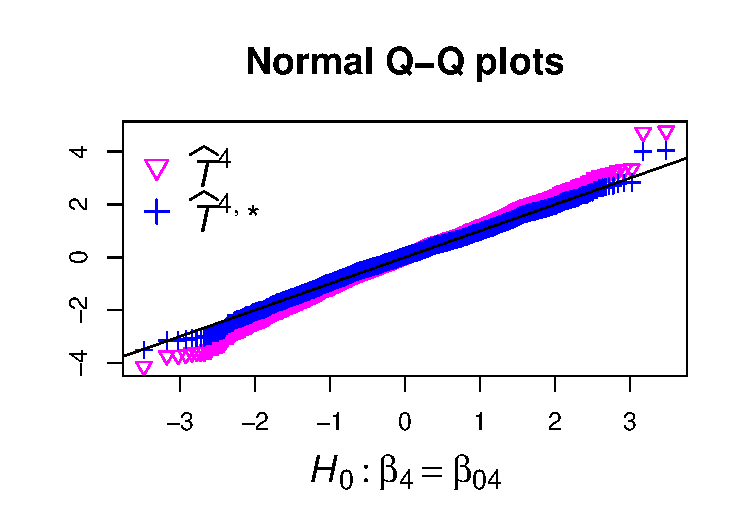
\includegraphics[width=12cm]{qq-clot.pdf}
	
	\caption{\label{qq-clot}Normal Q-Q plots based on 2000 values of $\widehat{T}^4$ and $\widehat{T}^{4,*}$ computed under the null hypothesis $H_0\!:\beta_4=\beta_{04}$ in the \emph{clotting} example.}
\end{figure}

\section{Title of section}
\noindent

% Chapter 3
\chapter{Akaike's information Criterion}

\fancyhead[RO,LE]{\thepage}
\fancyhead[LO]{Chapter 3 - \emph{Title of chapter}}
\fancyhead[RE]{Section \thesection \ - \emph{\Sectionname}}

\setlength{\parskip}{0.5pt}

\bigskip

\section{Kullback Leibler divergence } 
\noindent
\cite{azzalini01}

\section{AIC }
\noindent
\cite{bart53}

\subsection{Title of subsection}
\noindent
\cite{brglm2}

\subsection{Title of subsection}
\noindent
\cite{staf92}

\subsection{Title of subsection}
\noindent
\cite{dicicciostern93}

\section{AIC with quasi-likelihood function}
\noindent

\cleardoublepage
%%----------------------------------------------------------------
% Now begin the Appendices, including them as separate files

\addtocontents{toc}{\vspace{1em}} % Add a gap in the Contents, for aesthetics
\appendixtocoff
\appendixtitleon

\pagestyle{fancy}

% Cue to tell LaTeX that the following 'chapters' are Appendices
\begin{appendices}
	\renewcommand\thechapter{}

\chapter{}
\setcounter{equation}{0}
\renewcommand{\theequation}{A.\arabic{equation}}
\fancyhead[RO,LE]{\thepage}
\fancyhead[LO]{Appendix}
\fancyhead[RE]{Appendix}


\setlength{\parskip}{0.5pt}
\vspace{-2em}
%\bigskip
\noindent
 


	% Appendix Title
\end{appendices}
\clearpage
\pagestyle{empty}

\addtocontents{toc}{\vspace{1em}}  % Add a gap in the Contents, for aesthetics

\backmatter
%% ----------------------------------------------------------------

\bibliographystyle{CUP}
\pagestyle{fancy}
\label{Bibliography}
\fancyhead[RO,LE]{\thepage}
\fancyhead[LO]{Bibliography}
\fancyhead[RE]{Bibliography}
\bibliography{References/references}

\newpage
\thispagestyle{empty}
\mbox{}

\pagestyle{empty}
%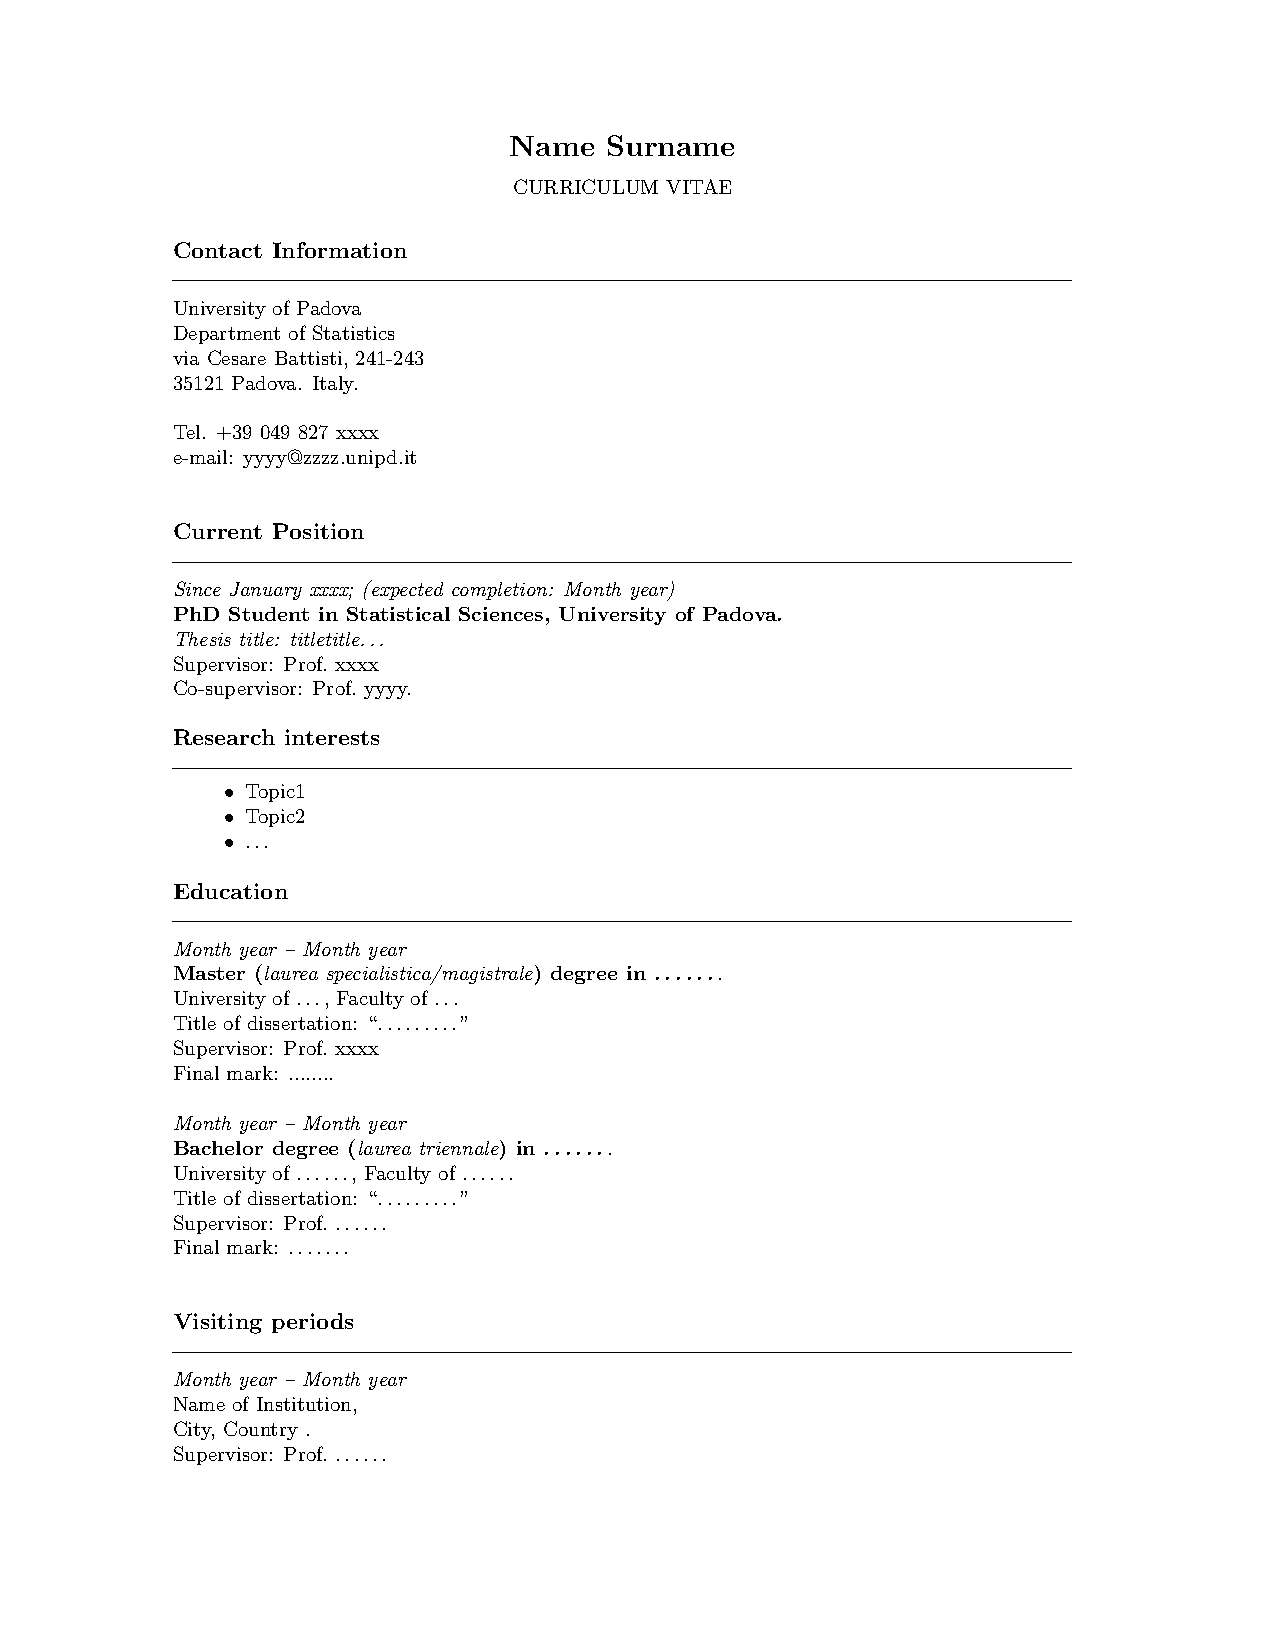
\includepdf[pages={1}, scale=1, offset=-3cm -2cm]{CVthesis/cv.pdf}
%\includepdf[pages={2}, scale=1, offset=-1.75cm -1.2cm]{CVthesis/cv.pdf}
%\includepdf[pages={3}, scale=1, offset=3cm -2cm]{CVthesis/cv.pdf}
%\includepdf[pages={4}, scale=1, offset=-1.75cm -1.2cm]{CVthesis/cv.pdf}
\end{document}  % The End
%%----------------------------------------------------------------